\documentclass[english,9pt,aspectraio=169]{beamer}
\usepackage{etex}
\usetheme{uzhneu-en-informal}
%\usepackage{uarial}
\usepackage[T1]{fontenc}
\usepackage[utf8]{inputenc}
\RequirePackage{graphicx,ae}
\usepackage{bm}
\usepackage{fancybox,amssymb,color}
\usepackage{pgfpages}
\usepackage{booktabs}
\usepackage{verbatim}
\usepackage{animate}
\usepackage{numprint}
\usepackage{dsfont}
\usepackage{tikz}
\usepackage{amsmath,natbib}
\usepackage{mathbbol}
\usepackage{babel}
\usepackage{SweaveSlides}
\usepackage{multicol}


\usetheme{uzhneu-en-informal}
\DeclareMathOperator{\po}{Poisson}
\DeclareMathOperator{\G}{Gamma}
\DeclareMathOperator{\Be}{Beta}
\DeclareMathOperator{\logit}{logit}
\def\n{\mathop{\mathcal N}}

\definecolor{Gray}{RGB}{139,137,137}
\definecolor{darkred}{rgb}{0.8,0,0}
\definecolor{Green}{rgb}{0,0.8,0.3}
\definecolor{Blue}{rgb}{0,0,1}
\def\myalert{\textcolor{darkred}}
\def\myref{\textcolor{Gray}}
\setbeamercovered{invisible}

\renewcommand{\baselinestretch}{1.2}
\beamertemplateballitem
\DeclareMathOperator{\cn}{cn} % Copy number
\DeclareMathOperator{\ccn}{ccn} % common copy number
\DeclareMathOperator{\p}{p} % common copy number
\DeclareMathOperator{\E}{E} % common copy number
\DeclareMathOperator{\given}{|} % common copy number
\def\given{\,|\,}
\def\na{\tt{NA}}
\def\nin{\noindent}
\pdfpageattr{/Group <</S /Transparency /I true /CS /DeviceRGB>>}
\def\eps{\varepsilon}

\renewcommand{\P}{\operatorname{\mathsf{Pr}}} % Wahrscheinlichkeitsmaß
\def\eps{\varepsilon}
\def\logit{\text{logit}}
%\newcommand{\E}{\mathsf{E}} % Erwartungswert
\newcommand{\Var}{\text{Var}} % Varianz
\newcommand{\NBin}{\text{NBin}}
\newcommand{\Po}{\text{Po}}


\newcommand{\ball}[1]{\begin{pgfpicture}{-1ex}{-0.65ex}{1ex}{1ex}
\usebeamercolor[fg]{item projected}

{\pgftransformscale{1.75}\pgftext{\normalsize\pgfuseshading{bigsphere}}}
{\pgftransformshift{\pgfpoint{0pt}{0.5pt}}
\pgftext{\usebeamerfont*{item projected}{#1}}}
\end{pgfpicture}}%
\usepackage{multicol}
\newcommand{\ballsmall}[1]{\begin{pgfpicture}{-1ex}{-0.65ex}{.2ex}{.2ex}
\usebeamercolor[fg]{item projected}

{\pgftransformscale{1}\pgftext{\normalsize\pgfuseshading{bigsphere}}}
{\pgftransformshift{\pgfpoint{0pt}{0.5pt}}
\pgftext{\usebeamerfont*{item projected}{#1}}}
\end{pgfpicture}}%


\begin{document}

\frame{
\title[]{ \centering \Huge Course Bio144: \\
Data analysis in biology}%\\[.3cm]
\author[Stefanie Muff, Owen L.\ Petchey]{\centering Stefanie Muff (Lectures) \& Owen L.\ Petchey (Exercises)}
\date[]{Lecture 1: Introduction and Outlook\\ 23./24. February 2017}


\maketitle
}



\frame{\frametitle{Organization}
To do:
\begin{itemize}
\item Testate conditions
\item Examination date
\item Link to course webpage
\end{itemize}

}


\frame{\frametitle{Literature}
Compulsory literature:
\begin{enumerate}[1.]
\item \emph{Lineare Regression} by W. Stahel (pdf on course webpage)
\item \emph{Getting Started With R} by A.P. Beckerman und O.L. Petchey, Oxford University Press;
ISBN 978-0-19-960162-2
\item \emph{The New Statistics With R} by A. Hector, Oxford University Press;
ISBN 978-0-19-872906-8 \\[5mm]
\end{enumerate}

\begin{center}

\includegraphics[width=3cm]{pictures/petchey_buch.jpeg} \qquad \qquad

\includegraphics[width=3cm]{pictures/hector.jpeg}
\end{center}

}

\frame{
\frametitle{Complementary literature:}
\begin{itemize}
\item \emph{Statistics – An Introduction Using R} by M.J. Crawley (similar to 3.) above)\\[3mm]
\item \emph{The Analysis of Biological Data} by M.C. Whitlock and D. Schluter\\[3mm]
\item \emph{Regression - Modelle, Methoden und Anwendungen} by Fahrmeier, Kneib, Lang
\end{itemize}
}

\frame{\frametitle{Overarching goals of the course}
 






\begin{itemize}
\item Provide a solid foundation for answering biological questions with quantitative data.\\[3mm]
\item Help students to understand the language of a statistician.\\[3mm]
\item Ability to understand and interpret results in research articles.\\[3mm]
\item Give the students a challenging, engaging, and enjoyable learning experience.\\[7mm]
\end{itemize}

My belief: A solid foundation in statistics makes you independent!  \\[2mm]

}

\frame{\frametitle{Prerequisite for Bio144}
\begin{itemize}
\item Mat183 ``Stochastik f\"ur die Naturwissenschaften'' (2nd semester)
\end{itemize}

}



\frame{\frametitle{Schedule (14 weeks, 12 lectures)}
\vspace{-8mm}

\begin{multicols}{2}
1. Introduction and outlook \\[1mm]
2. Simple linear regression\\[1mm]
3. Residual analysis, model validation\\[1mm]
4. Multiple linear regression \\[1mm]
5. ANOVA and ANCOVA \\[1mm]
6. Matrix Algebra \\[1mm]
7. Model choice  \\[1mm]
8. Self-study week \\[1mm]
9. Interpretation of the results \\[1mm]
10. Binary Data (logistic regression)\\[1mm]
11. Count data (Poisson regression) \\[1mm]
12. Measurement error, random effects \\[1mm]
13. Self-study week \\[1mm]
14. Selected topics, repetition and outlook \\
\end{multicols}
~\\
{\bf Short-dated changes possible!}
}

\frame{\frametitle{Why is statistical data analysis so relevant for the biological and medical sciences?}

What do you think? \\[4mm]



\pause

Awareness that, without a profound knowledge in statistical data analysis, it will be hard to analyze your data from Bachelor, Master or PhD theses.... \\[2mm]

Examples:
\begin{itemize}
\item Medicine: Does a drug have a positive effect? Which factors cause cancer?
\item Ecology: What is a suitable habitat for a certain animal? Which resources does it need or prefer?
\item Evolutionary biology: Do highly inbred animals have decreased chances to survive or reproduce?
\end{itemize}
}

\frame{
Be careful! "Learning by doing" is not advisable in statistics. Experience is essential, there are many pitfalls.\\[5mm]

A good foundation in statistics makes you more independent from consultants or the goodwill of colleagues. Without such a knowledge, you will always need help from others.\\[5mm]

Data analysis is itself an exciting part of research! \\[5mm]
 
Data analysis is at the interface between mathematics and biology (and other research fields such as medicine, earth sciences, and so on).

}


\frame{\frametitle{What are the purposes of data analysis?}
\begin{itemize}
\item To find and quantify associations through graphical representations and modelling.\\[3mm]
\item To draw conclusion from data.\\[3mm]
\item To quantify the uncertainty of these conclusions.\\
\end{itemize}
}

\frame{\frametitle{Own examples}
\myalert{\large Otter (lutra lutra)} \citep{weinberger.etal2016}\\[2mm]

\emph{Research questions:} What is the preferred habitat by otters? How do otters adapt to human altered landscapes? \\[1mm]
\emph{Method:} Study in Austria, 9 Otter were radio-tracked and monitored during 2-3 years.\\


\includegraphics[width=10cm]{pictures/otters.jpeg}
}


\frame{
\myalert{\large Inbreeding in Alpine ibex}\\[2mm]

\emph{Research question:} Does inbreeding in Alpine ibex populations have a negative effect on long-term population growth? Inbreeding depression!\\[4mm]

\begin{multicols}{2}
\emph{Methods:} Genetic information from blood samples allow to quantify the level of inbreeding in each ibex population. In addition, long-term monitoring of population sizes and harvest rates.\\[3mm]

%\begin{center}
%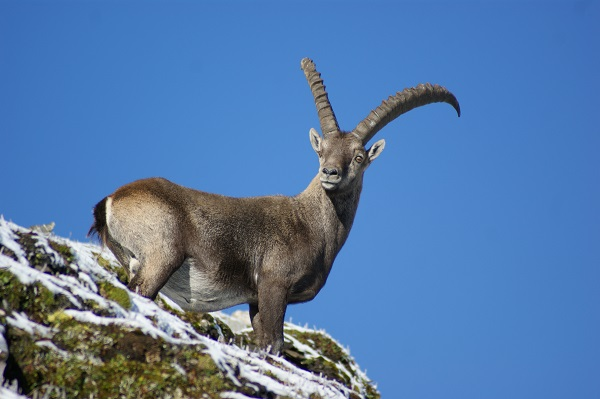
\includegraphics[width=4cm]{pictures/steinbock.jpg} \hspace{1cm}
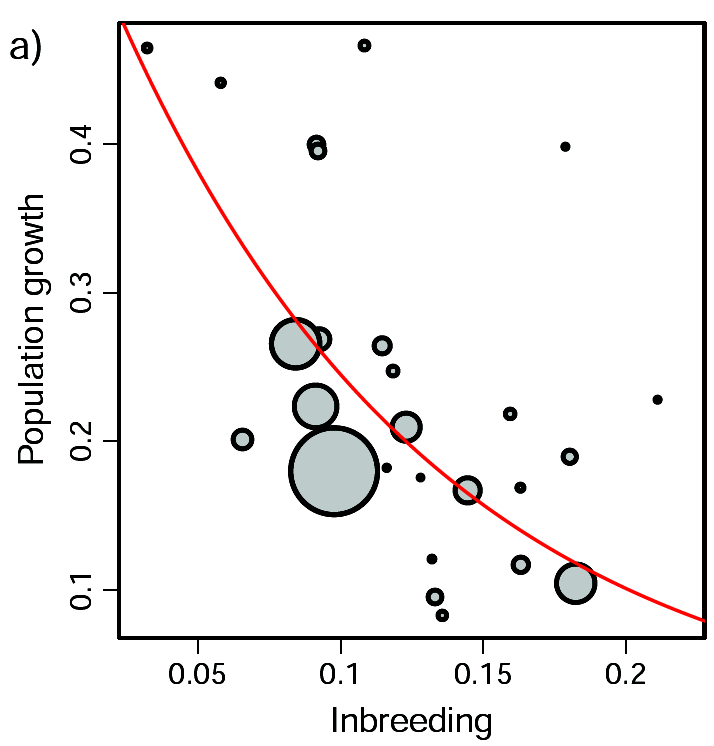
\includegraphics[width=4cm]{pictures/ibex_graph.png}
%\end{center}
\end{multicols}
\vspace{-1cm}
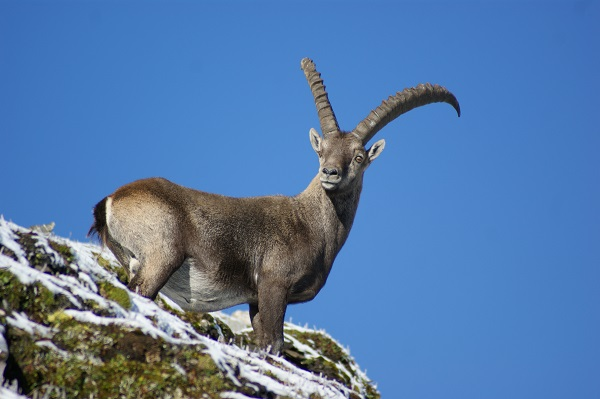
\includegraphics[width=3cm]{pictures/steinbock.jpg}
}

\frame{\frametitle{}
\myalert{Mercury (Hg) in the soil} \\[2mm]

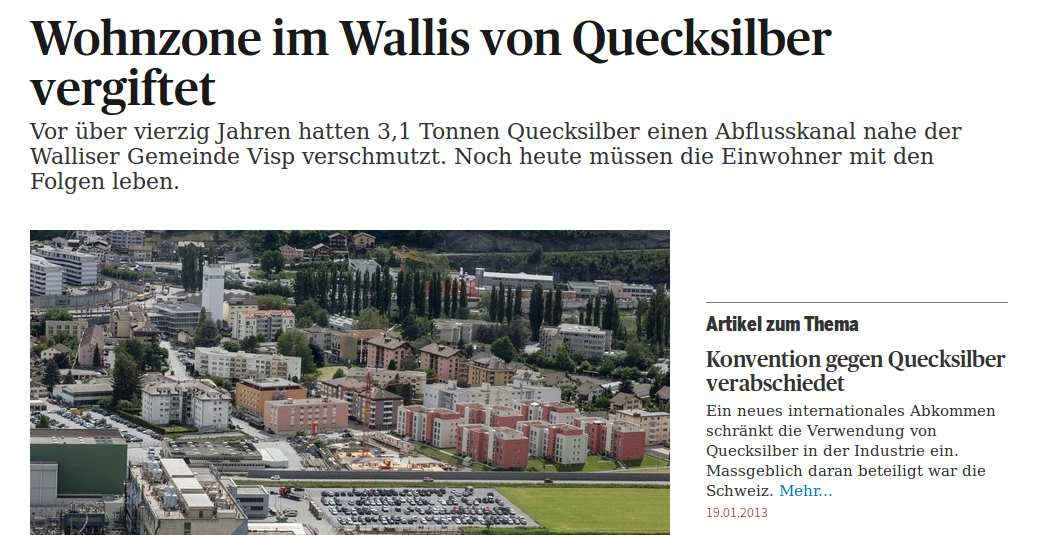
\includegraphics[width=8cm]{pictures/wallis.png} \\[2mm]

\emph{Research question:} Is the Hg level in the environment (soil) of people's homes associated to the Hg levels in their bodies (urin, hair)?\\[2mm]
\emph{Method:} Measurements of Hg concentrations on people's properties, as well as measurements and survey of children and their mothers living in these properties.\\[2mm]

Highly delicate, emotionally charged, political question!\\
\href{http://www.srf.ch/news/regional/bern-freiburg-wallis/quecksilber-im-walliser-boden-schadete-der-gesundheit-nicht}
{\beamergotobutton{Schweiz Aktuell, 20. Juni 2016}}
 
}


\frame{\frametitle{}
\myalert{Physical activity in children} \\[6mm]

%\includegraphics{pictures/g}

\emph{Research question:} Which factors influence physical activity patterns in children aged 2-6 years?\\[4mm]

\emph{Method:} The children had to wear accelerometers for several days. In addition, their parents had to fill in a detailed questionnaire.\\[4mm]
Observed variables were, e.g., media consumption, behavior of the parents, age, weight, social structure,...\\[7mm]



\href{http://splashy.ch/}
{\beamergotobutton{Link to Splashy study}}
 
}



\frame{\frametitle{Statistics in the news (April 2016)}
 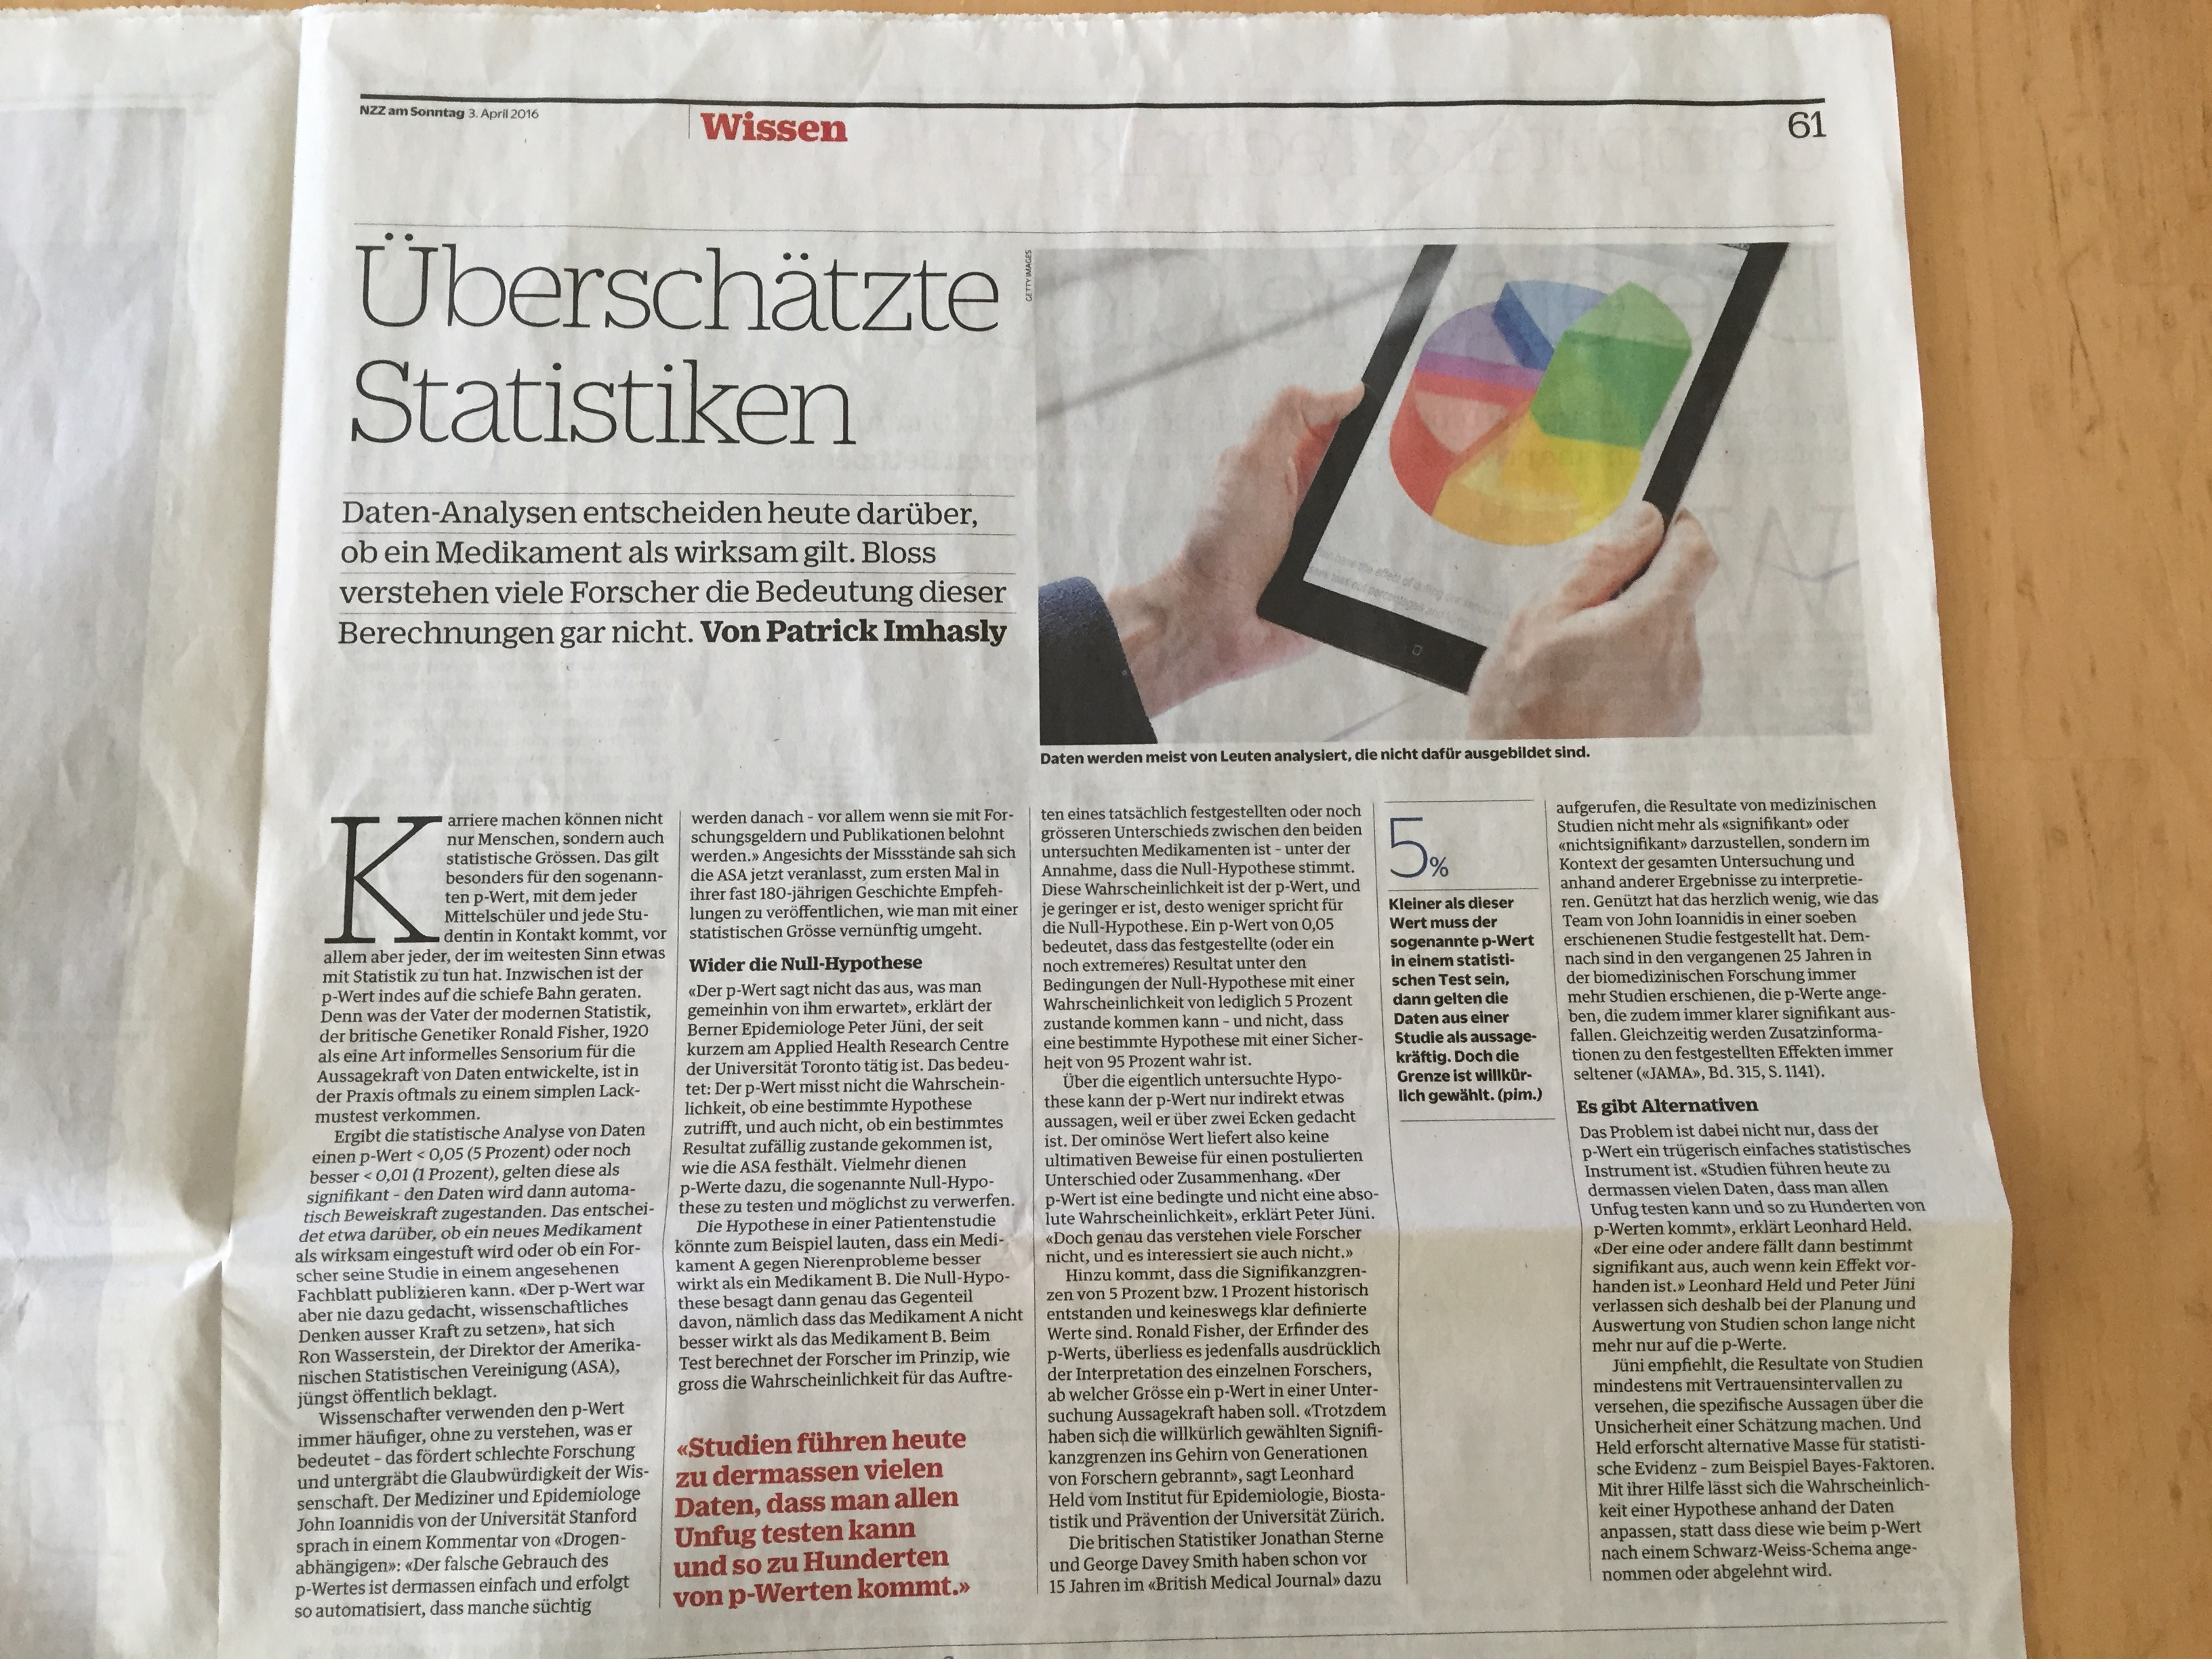
\includegraphics[width=9cm]{pictures/NZZ1.jpeg}\\
\url{https://www.theguardian.com/science/2016/jul/17/politicians-dodgy-statistics-tricks-guide?&tc=eml}
}


\frame[containsverbatim]{\frametitle{Data example 1: Prognostic factors for body fat}
\vspace{-1cm}
{\scriptsize (From Theo Gasser \& Burkhardt Seifert \emph{Grundbegriffe der Biostatistik})}\\[6mm]

Body fat is an important indicator for overweight, but difficult to measure. \\
{\bf Question:}  Which factors allow for precise estimation (prediction) of body fat? \\[4mm]

Study with 241 male participants. Measured variable were, among others, body fat (\%), age, weight, body size, BMI, neck thickness and abdominal girth.\\[4mm]

\begin{Schunk}
\begin{Sinput}
> str(d.bodyfat)
\end{Sinput}
\begin{Soutput}
'data.frame':	243 obs. of  7 variables:
 $ bodyfat: num  12.3 6.1 25.3 10.4 28.7 20.9 19.2 12.4 4.1 11.7 ...
 $ age    : int  23 22 22 26 24 24 26 25 25 23 ...
 $ gewicht: num  70 78.7 69.9 83.9 83.7 ...
 $ hoehe  : num  172 184 168 184 181 ...
 $ bmi    : num  23.6 23.4 24.7 24.9 25.5 ...
 $ neck   : num  36.2 38.5 34 37.4 34.4 39 36.4 37.8 38.1 42.1 ...
 $ abdomen: num  85.2 83 87.9 86.4 100 94.4 90.7 88.5 82.5 88.6 ...
\end{Soutput}
\end{Schunk}
 

}


\frame[containsverbatim]{\frametitle{}
 
\setkeys{Gin}{width=0.75\textwidth}
\begin{Schunk}
\begin{Sinput}
> pairs(d.bodyfat)
\end{Sinput}
\end{Schunk}
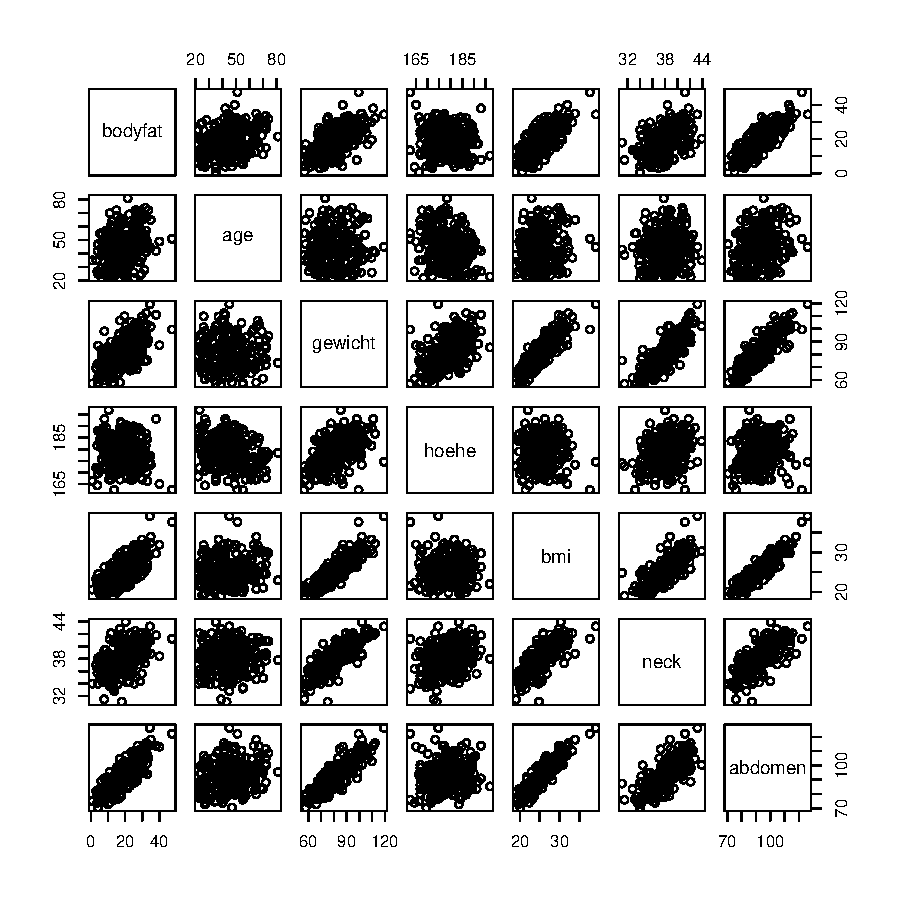
\includegraphics{Bio144_2017_lecture1-pairs}

\texttt{pairs()} gives us the scatterplots of all against all variables.
}



\frame{\frametitle{}
\vspace{-0.5cm}
\begin{center}
\setkeys{Gin}{width=0.7\textwidth}
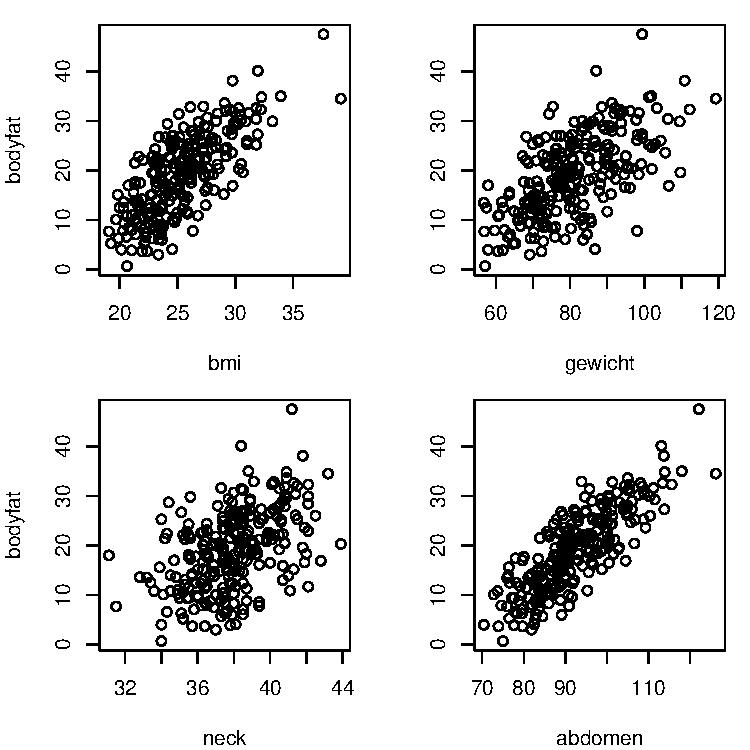
\includegraphics{Bio144_2017_lecture1-004}
\end{center}

We are looking for a \emph{model} that \myalert{predicts} body fat as precisely as possible from variables that are easy to measure. 
}



\frame[containsverbatim]{\frametitle{Data example 2: Mercury in Valais (Switzerland)}
{\bf Question:} Association between Hg concentrations in the soil and in the urin of the people living in the respective properties. We use a slightly modified data set here.\\[5mm]

\begin{Schunk}
\begin{Sinput}
> str(d.hg)
\end{Sinput}
\begin{Soutput}
'data.frame':	156 obs. of  10 variables:
 $ Hg_urin       : num  0.258 0.036 0.16 0.314 0.29 ...
 $ Hg_soil       : num  0.49 0.42 0.18 0.49 0.24 0.2 0.1 14 0.1 0.3 ...
 $ veg_garden    : int  1 1 1 1 1 1 1 1 1 1 ...
 $ migration     : int  0 0 0 0 0 0 0 0 0 0 ...
 $ smoking       : int  0 0 0 0 0 0 0 0 0 0 ...
 $ amalgam       : int  3 0 2 0 0 0 0 1 0 0 ...
 $ age           : int  51 11 34 8 6 40 7 48 11 38 ...
 $ fish          : int  3 2 5 4 4 2 2 4 0 7 ...
 $ last_time_fish: int  0 0 0 0 0 0 0 0 0 0 ...
 $ mother        : Factor w/ 2 levels "0","1": 2 1 2 1 1 2 1 2 1 2 ...
\end{Soutput}
\end{Schunk}

}


\frame[containsverbatim]{\frametitle{}
\vspace{1cm}
A first visual inspection is not very informative. There is no association visible by eye:
%
\begin{center}
\setkeys{Gin}{width=0.65\textwidth}
\begin{Schunk}
\begin{Sinput}
> plot(Hg_urin ~ Hg_soil, data=d.hg, xlab="Hg soil", ylab = "Hg Urin")
\end{Sinput}
\end{Schunk}
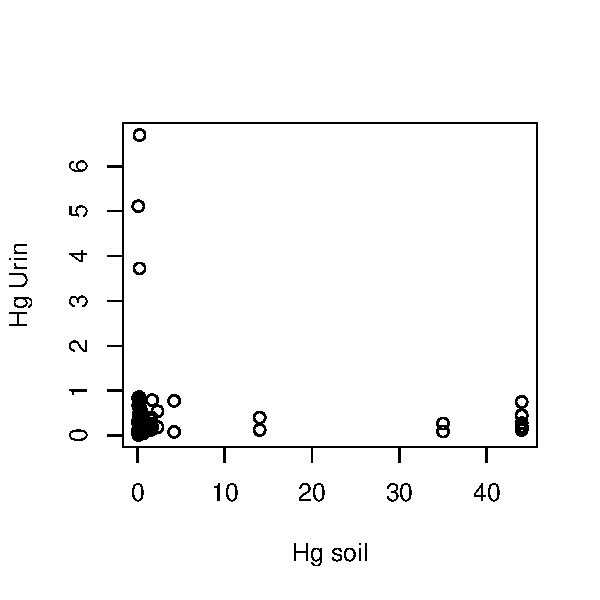
\includegraphics{Bio144_2017_lecture1-hg1}
\end{center}

}

\frame[containsverbatim]{\frametitle{}
Which other factors might be responsible for high Hg concentrations in urin?\\[4mm]

\begin{center}
\setkeys{Gin}{width=1.0\textwidth}
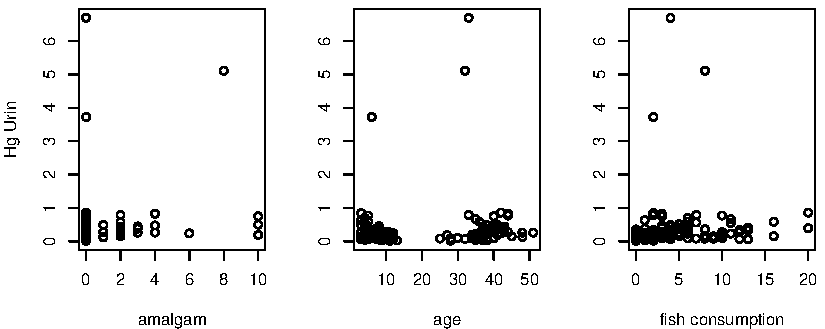
\includegraphics{Bio144_2017_lecture1-hg2}
\end{center}
\vspace{5mm}

From these plots it is hard to tell which factors exactly influence the Hg pollution in humans.

}


\frame[containsverbatim]{\frametitle{}
It is always useful to look at the distribution of the variables in the model. Let us plot the histogram of Hg concentrations:\\[4mm]

\begin{center}
\setkeys{Gin}{width=0.9\textwidth}
\begin{Schunk}
\begin{Sinput}
> par(mfrow=c(1,2))
> hist(d.hg$Hg_soil,xlab="Hg soil",nclass=20,main="")
> hist(d.hg$Hg_urin,xlab="Hg Urin",nclass=20,main="")
\end{Sinput}
\end{Schunk}
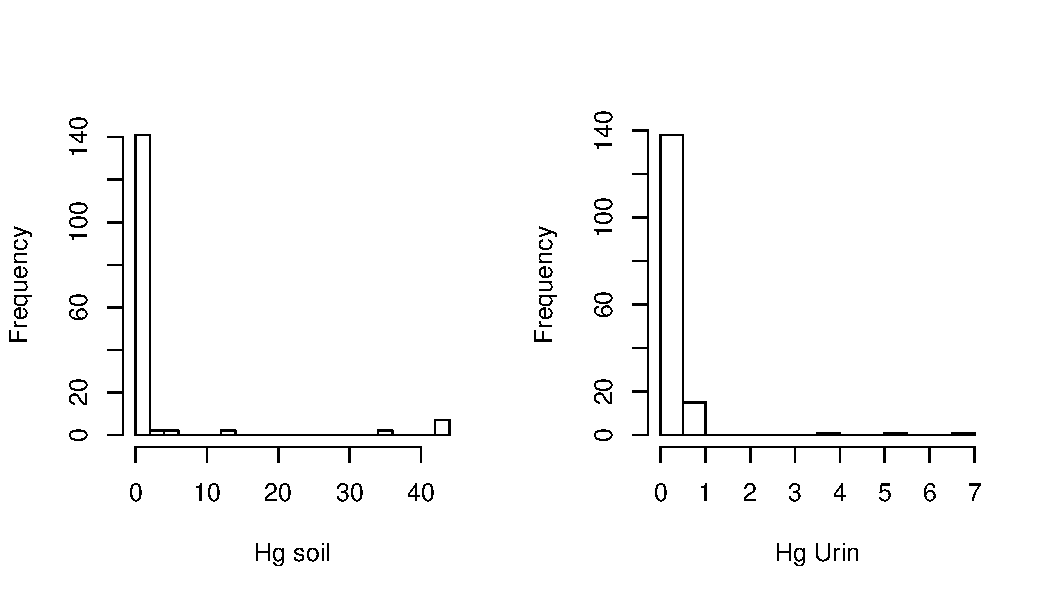
\includegraphics{Bio144_2017_lecture1-hghist}
\end{center}

All Hg values seem to ``stick'' at 0.


}

\frame[containsverbatim]{\frametitle{}
In such cases in can help to \emph{log-transform} the respective variables.

 \begin{center}
\setkeys{Gin}{width=0.9\textwidth}
\begin{Schunk}
\begin{Sinput}
> par(mfrow=c(1,2))
> hist(log(d.hg$Hg_soil),xlab="log(Hg soil)",nclass=20,main="")
> hist(log(d.hg$Hg_urin),xlab="log(Hg soil)",nclass=20,main="")
\end{Sinput}
\end{Schunk}
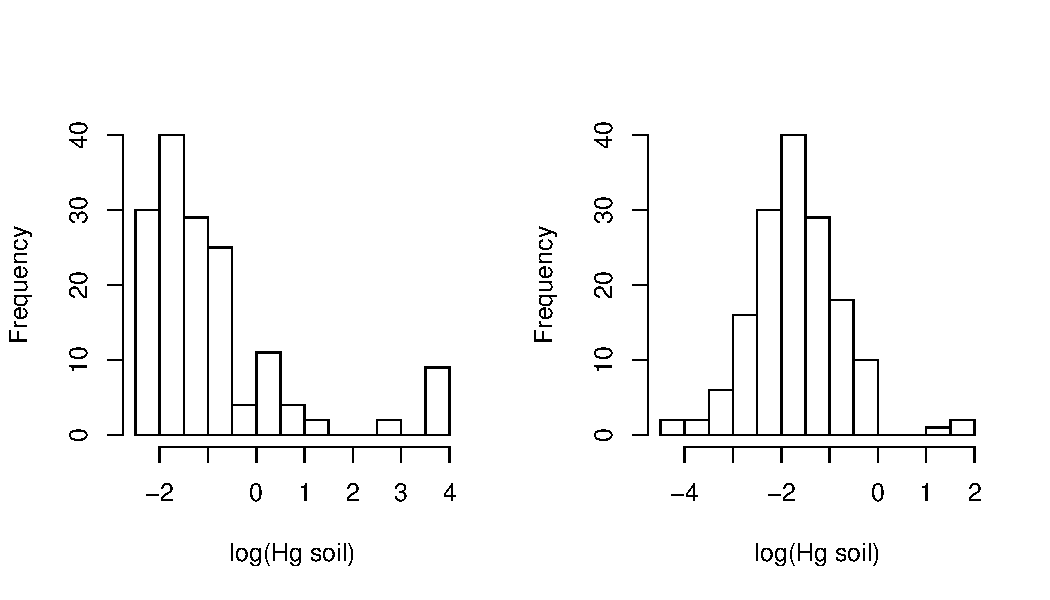
\includegraphics{Bio144_2017_lecture1-hghist2}
\end{center}
}

\frame[containsverbatim]{\frametitle{}
The scatterplot does also look much more reasonable with log-transformed values:

\begin{center}
\setkeys{Gin}{width=0.5\textwidth}
\begin{Schunk}
\begin{Sinput}
> plot(log(Hg_urin) ~ log(Hg_soil), data=d.hg, xlab="Hg soil", 
+      ylab = "Hg Urin",pch=21,bg=as.numeric(mother)+2,xlim=c(-4.5,4.5))
> legend("topright",legend=c("Children","Mothers"),col=c(3,4),pch=21,pt.bg=c(3,4))
\end{Sinput}
\end{Schunk}
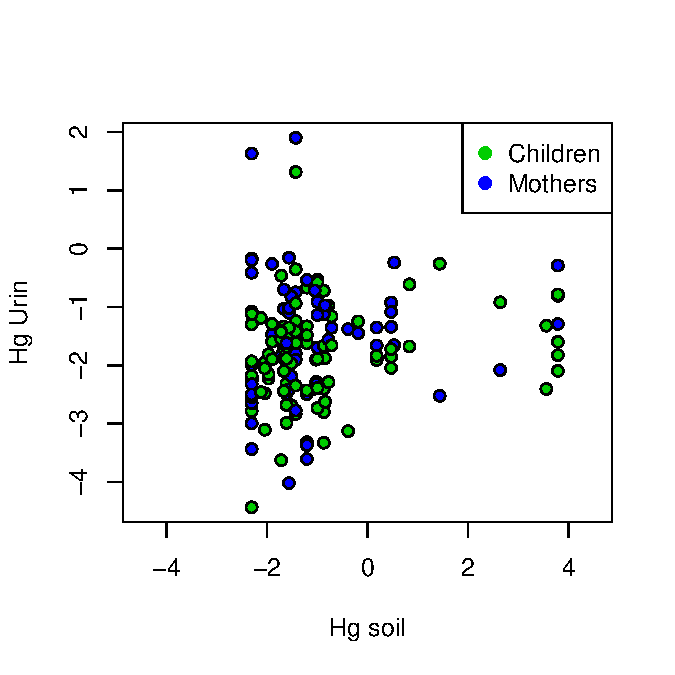
\includegraphics{Bio144_2017_lecture1-hg1_log}
\end{center}

Remember: The idea to log-transform the variables was mainly obvious thanks to \myalert{visual inspection}!

}





\frame[containsverbatim]{\frametitle{Data example 3: Diet and blood glucose level}
\vspace{-3mm}
{\scriptsize\citep[p. 190]{elpelt.hartung1987}}\\[2mm]
%
24 persons were split into 4 groups. Each group followed another diet \small{(DIAET)}. The blood glucose concentrations were measured at the beginning and at the end (after 2 weeks). The difference of these values was stored \small{(BLUTZUCK)}.\\[2mm]
{\bf Question:} Are there differences among the groups with respect to changes in blood glucose concentrations?\\[3mm]

\begin{center}
\setkeys{Gin}{width=0.7\textwidth}
\begin{Schunk}
\begin{Sinput}
> par(mfrow=c(1,2))
> plot(BLUTZUCK ~ DIAET,d.blz,xaxt="n",main="Scatterplot")
> axis(1,1:4)
> boxplot(BLUTZUCK ~ DIAET,d.blz,xaxt="n",xlab="DIAET",main="Boxplot")
> axis(1,1:4)
\end{Sinput}
\end{Schunk}
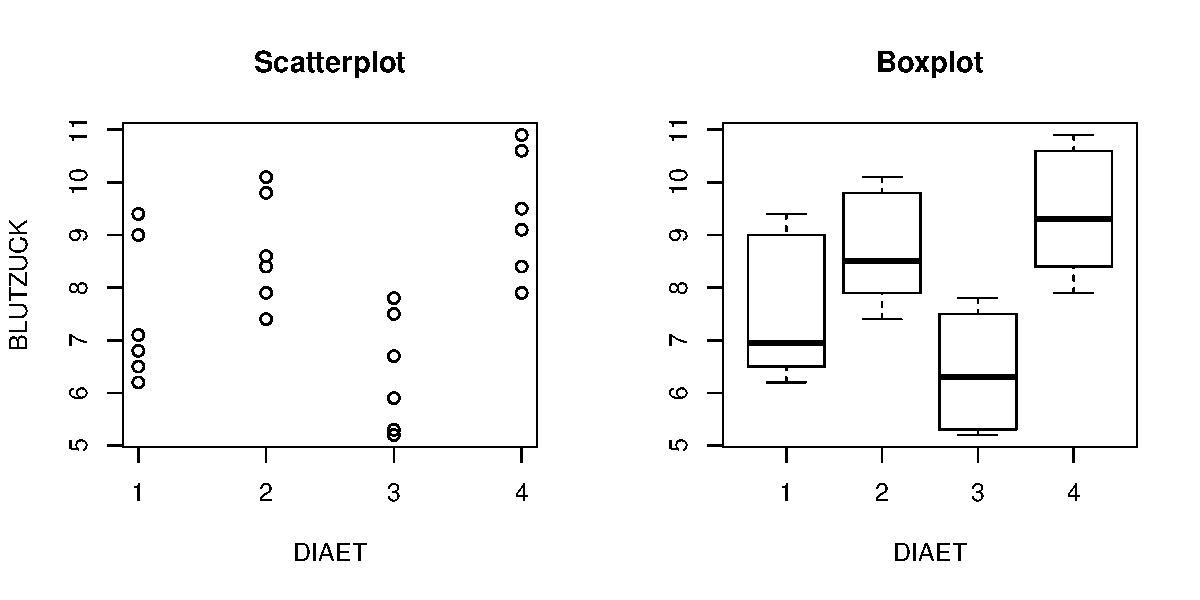
\includegraphics{Bio144_2017_lecture1-blz_plot}
\end{center}

}


\frame[containsverbatim]{\frametitle{}
Does this question seem familiar to you? \\
Hint: what would you do for two groups? \\[4mm]

For more than 2 groups we need the \emph{ANOVA} (=ANalysis Of VAriance) approach.\\[4mm]

We will see in week 5 that there are in fact differences between the diets. \\[4mm]

The next question then is: which diets are \emph{pairwise} different.

}

\frame[containsverbatim]{\frametitle{Data example 4: Blood-screening}
\vspace{-5mm}
{\scriptsize\citep[From ][Chapter 7.1]{hothorn.everitt2014}}\\[4mm]

Is a high ESR (erythrocyte sedimentation rate) an indicator for certain diseases (rheumatic disease, chronic inflammations)?\\[3mm]

{\bf  Specifically: } Is there an association between ESR level ESR$<20mm/hr$ and the concentrations of the plasma proteins Fibrinogen and Globulin?\\[3mm]

Load data from the package that comes with \citet{hothorn.everitt2014}:\\[2mm]

\begin{Schunk}
\begin{Sinput}
> library(HSAUR3)
> data("plasma",package="HSAUR3")
\end{Sinput}
\end{Schunk}
\begin{Schunk}
\begin{Sinput}
> plasma[c(1,5,9,10,15,29),]
\end{Sinput}
\begin{Soutput}
   fibrinogen globulin      ESR
1        2.52       38 ESR < 20
5        3.41       37 ESR < 20
9        3.15       39 ESR < 20
10       2.60       41 ESR < 20
19       2.60       38 ESR < 20
15       2.38       37 ESR > 20
\end{Soutput}
\end{Schunk}
}

\frame[containsverbatim]{\frametitle{}
The distinction ESR$<20mm/hr$ vs.\ ESR$\geq 20mm/hr$ leads to a \myalert{binary} variable.\\

The relation between the plasmaprotein levels and the binary indicator can be captured by a \emph{conditional density plot}.

\begin{center}
\setkeys{Gin}{width=0.9\textwidth}
\begin{Schunk}
\begin{Sinput}
> par(mfrow=c(1,2))
> cdplot(ESR ~ fibrinogen,plasma)
> cdplot(ESR ~ globulin,plasma)
\end{Sinput}
\end{Schunk}
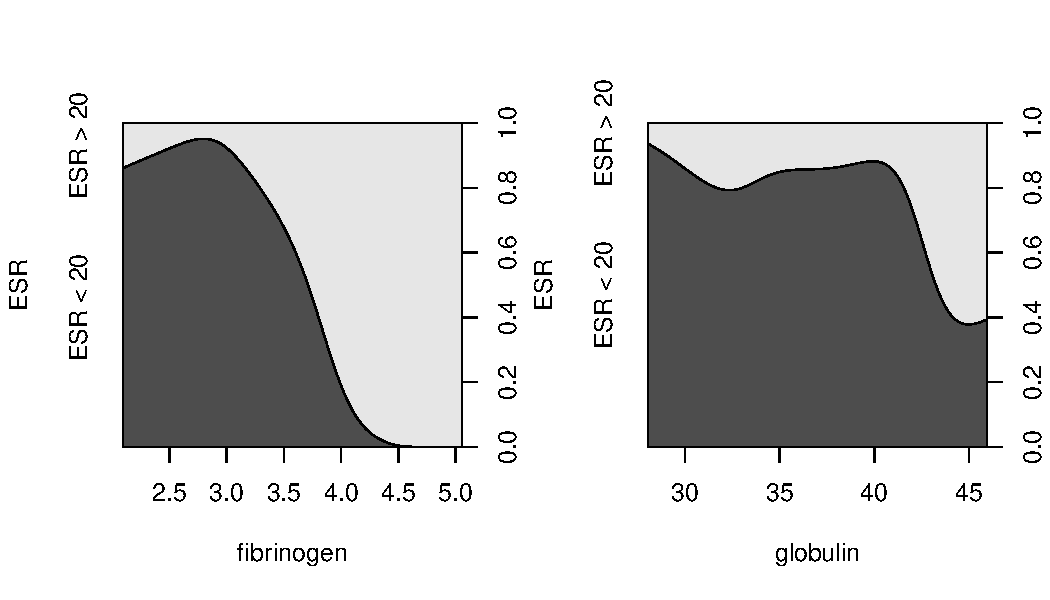
\includegraphics{Bio144_2017_lecture1-cdplot_ESR}
\end{center}

}


\frame{\frametitle{What is a model?}
A model is an approximation of the reality. Understanding how the real world works is usually only possible thanks to simplifying assumptions. This is exactly the purpose of statistical data analysis.\\[6mm]

In 2014, David Hand wrote:\\[4mm]

\emph{In general, when building statistical models, we must
not forget that the aim is to understand something about
the real world. Or predict, choose an action, make
a decision, summarize evidence, and so on, but always
about the real world, not an abstract mathematical
world: our models are not the reality -- a point well
made by George Box in his oft-cited remark that \myalert{``all
models are wrong, but some are useful'' \citep{box1979}.}
}

}


\frame{\frametitle{Steps in a modelling process}
\begin{enumerate}
\item Formulate a precise question
\item Plan your inquiry and the analysis of your data, collect the data (experiments or surveys).
\item Tidy and clean the data
\item Graphical representation of the data
\item Choose an appropriate \emph{model}
\item Estimate model parameters and uncertainties
\item Check modelling assumptions
\item If needed, improve the model; back to step 7
\item Interpret your results and compare to step 1
\item Communicate results precisely and carefully (publication, articles..)
\end{enumerate}

}


\frame{\frametitle{The scopes of statistical data analysis}
\begin{enumerate}[a)]
\item \myalert{Prediction, interpolation}. Example body fat: use substitute measurements to predict body fat of a person.\\[3mm]
\item \myalert{Estimation of parameters.} \\[3mm]
\item \myalert{Determine important variables}. Example physical activity of children: The study aims to find factors that (positively or negatively) influence the movement behavior of children. \\[3mm]
\item Optimization. \\[3mm]
\item Calibration.\\[8mm]
\end{enumerate}

In this course we are concerned with a)-c).
}

\frame{\frametitle{Goals of the course (part 2)}
By the end of the course you will be able analyze all data examples introduced here (and of course many more), as well as to draw conclusions from them.

}


\frame[containsverbatim]{\frametitle{Graphical representation of data}
You should remember the following options for graphical data descriptions. Several of them appeared already in previous examples.\\[4mm]

\begin{tabular}{ll}
Representation & Useful for \\
\hline
 Scatterplots & Pairwise dependency of continuous \\
    &  variables. \\[1mm]
 Histograms & Distribution of numerical variables.\\[1mm]
 Boxplots  & Distribution of numerical variables, ev. \\
    & conditionally on categories.\\[1mm]
 Conditional density plots &  Dependency of a binary variable from\\
    &  a continuous variable.\\[1mm]
Barplots & As boxplots. \\[1mm]
Coplots & Dependencies among multiple variables. \\
\hline
\end{tabular}


}


\frame[containsverbatim]{\frametitle{Barplots}
Examples from Beckerman \& Petchey: \\[2mm]
{\bf Left:} Fruit production in grazed and ungrazed areas. Grazing reduces above-ground biomass. How is fruit production affected by this?\\[2mm]
{\bf Right:} Number of birds of certain colors in two environments.

\begin{center}
\setkeys{Gin}{width=0.8\textwidth}
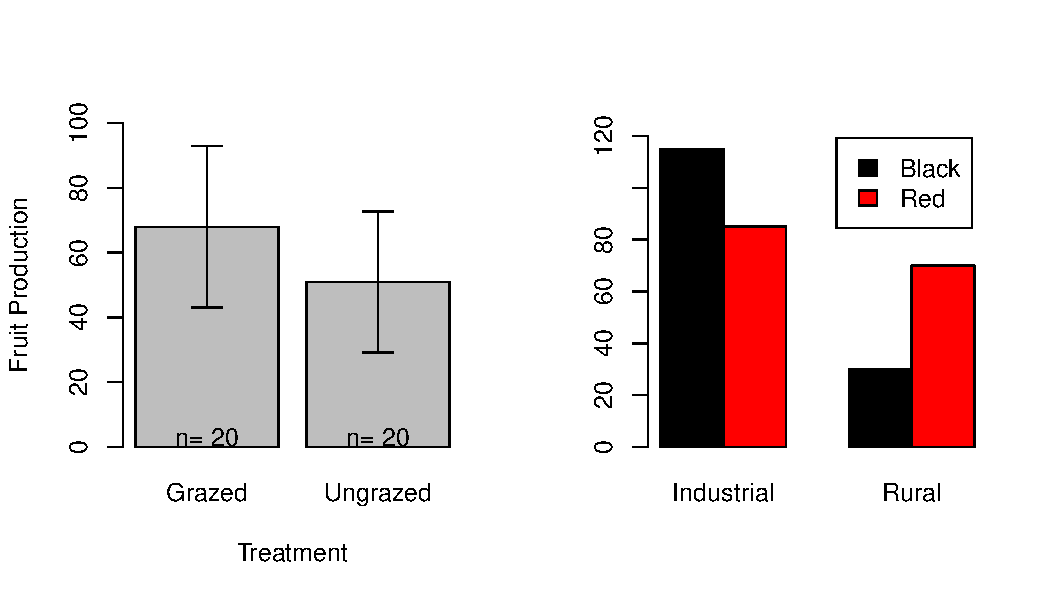
\includegraphics{Bio144_2017_lecture1-017}
\end{center}
}

\frame[containsverbatim]{\frametitle{Coplots}
Ideal to graphically display dependencies when more than two variables are involved. Very useful for categorical variables. Example: Mercury in Valais.

\begin{center}
\setkeys{Gin}{width=0.7\textwidth}
\begin{Schunk}
\begin{Sinput}
> coplot(log(Hg_urin) ~  age | mother * migration ,d.hg,panel=panel.smooth)
\end{Sinput}
\end{Schunk}
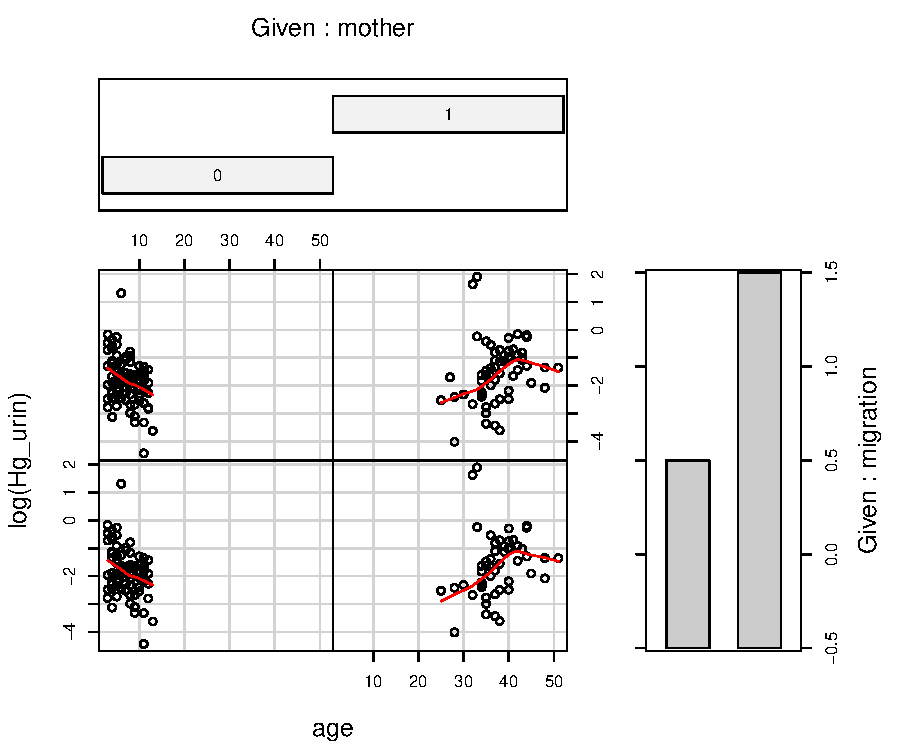
\includegraphics{Bio144_2017_lecture1-coplot}
\end{center}

}

\frame[containsverbatim]{\frametitle{}
There are many ``fancy'' ways to graphically display data ({\bf nice-to-know}):

\begin{itemize}
\item 3D-plots\\[1mm]
\item Spatial representations (using geodata)\\[1mm]
\item Interactive graphs and animations\\[6mm]
\end{itemize}

Many R packages are available for various purposes. Interactive apps can, for example, be generated with Shiny (see census app).


%' <<>>=
%' library(shiny)
%' runApp("/home/steffi/Shiny/Tutorial/census-app")
%' @
}

\frame{\frametitle{Experimental vs observational data}
To do, ev mention only later in weeks 7/8}

\frame{\frametitle{Next week: Simple linear regression}

}



\frame{References:
\bibliographystyle{Chicago}
\bibliography{refs}
}




%\frame[containsverbatim]{\frametitle{Conditional density plots}
%Ideal, um Einfluss einer kontinuierlichen Variable auf einen bin\"aren Outcome (z.B. krank ja/nein) darzustellen
%\begin{center}
%<<echo=T>>=
%par(mfrow=c(1,1))
%fail <- factor(c(2, 2, 2, 2, 1, 1, 1, 1, 1, 1, 2, 1, 2, 1, 1, 1,1, 2, 1, 1, 1, 1, 1),
%               levels = 1:2, labels = c("no", "yes"))
%temperature <- c(53, 57, 58, 63, 66, 67, 67, 67, 68, 69, 70, 70,
%                 70, 70, 72, 73, 75, 75, 76, 76, 78, 79, 81)
%@
%\setkeys{Gin}{width=0.5\textwidth}
%<<cdplot,fig=T,echo=T,width=4,height=4>>=
%cdens <- cdplot(fail ~ temperature)
%@
%\end{center}
%}


\end{document}
